\documentclass[12pt, a4paper, openany]{report}

\usepackage[utf8]{inputenc}
\usepackage[T1]{fontenc}
\usepackage{lmodern}
\usepackage{setspace}
\usepackage{amsmath, amssymb}
\usepackage{graphicx}
\usepackage{booktabs}
\usepackage{hyperref}
\usepackage{bookmark}
\usepackage{geometry}
\usepackage{caption}
\usepackage{subcaption}
\usepackage{tikz}
\usetikzlibrary{positioning, arrows.meta, shapes.geometric, fit, calc}
\usepackage{float}
\usepackage{enumitem}
\usepackage[numbers]{natbib}
\usepackage{multirow}
\usepackage{array}
\usepackage{titlesec}

\hypersetup{
  colorlinks=true,
  linkcolor=black,
  citecolor=black,
  urlcolor=black
}

\onehalfspacing

\geometry{
  a4paper,
  margin=1in
}

\titlespacing*{\chapter}{0pt}{-20pt}{15pt}

\graphicspath{{figures/}}

\begin{document}

\pagenumbering{roman}

% ---- Title Page ----
\begin{titlepage}
\centering
\vspace*{1.5cm}
{\Large \textbf{EE491-EE492\\Senior Design Project Midterm Report}}\\[2cm]
{\LARGE \textbf{Multi-Sensor Cough Analysis and State\\[0.3cm]
Classification with Machine Learning}}\\[3cm]
{\large \textbf{Submitted by:}\hspace{0.5em}Abdulhalim Kiraz}\\[1.5cm]
{\large \textbf{Principal Investigator:}\hspace{0.5em}Prof.\ Dr.\ Yasemin Kahya}\\[3cm]
\vfill
{\large 06.04.2026}
\end{titlepage}

% ---- Acknowledgments ----
\chapter*{ACKNOWLEDGMENTS}
\addcontentsline{toc}{chapter}{ACKNOWLEDGMENTS}
\begin{itemize}
\item I would like to express my sincere gratitude to Prof.\ Dr.\ Yasemin Kahya for her guidance, valuable feedback, and continuous support throughout this project.
\item I also thank Onur Yusuf \c{C}{\i}nar for providing the dataset used in this study and for his assistance during the data preparation process.
\end{itemize}

% ---- Abstract ----
\chapter*{ABSTRACT}
\addcontentsline{toc}{chapter}{ABSTRACT}
This report presents deep learning models for cough detection and activity classification using wearable multi-sensor data. The system uses four synchronized sensor channels: a pulmonary microphone, an ambient microphone, a stretch sensor, and an accelerometer. Three model versions were developed and compared. The first version (V1) uses a dual-branch 1D convolutional neural network that processes raw audio and motion signals separately and combines them through late fusion. The second version (V2) introduces center-focused window labeling, data augmentation, and learning rate scheduling while keeping the same architecture. The third version (V3) replaces the raw audio input with log-Mel spectrograms processed by a 2D CNN, while the motion branch stays unchanged. V3 achieved the best cough detection performance with 0.93 overall accuracy and 0.95 cough recall on the test set. Activity classification reached up to 0.92 accuracy with class weighting strategies. These results show that deep learning can detect coughs from multi-sensor wearable data without manual feature engineering.

% ---- Table of Contents ----
\tableofcontents

% ---- Chapters ----
\pagenumbering{arabic}
\chapter{INTRODUCTION}

\section{Background and Motivation}

Cough is an important physiological signal that provides information about respiratory health. Continuous cough monitoring can support early detection of respiratory diseases, help in treatment follow-up, and allow long-term patient observation. However, automatic cough detection in daily-life conditions is difficult due to background noise, motion artifacts, and privacy concerns with audio recordings~\cite{dixon2025}.

Wearable sensors offer an alternative to microphone-only systems. Body-coupled audio, accelerometers, and stretch sensors can capture cough events while being less affected by environmental noise~\cite{elfaramawy2017}. Still, these signals are noisy and depend on the user's activity. Both signal processing and data-driven methods are needed for reliable detection.

This project uses a wearable system with four sensors to detect cough events and classify the user's activity during coughing. In this phase, deep learning models are developed to learn patterns directly from the sensor signals, reducing the need for manual feature engineering.

\section{Previous Work}

In the first phase of this project (EE491), a classical machine learning pipeline was developed for the same task. Time-domain and frequency-domain features were extracted from short signal windows (200\,ms duration, 50\,ms hop), and classifiers such as Random Forest and XGBoost were trained using GroupKFold cross-validation with 5 folds. The dataset at that time included 60 recordings from a single subject.

The best cough detection model (XGBoost) achieved an event-level F1-score of 0.922 using IoU-based matching at a threshold of 0.20. Activity classification between sitting and walking reached 0.89 window-level accuracy with Random Forest.

While these results were promising, the approach required manual selection of features. The model performance was limited to what the handcrafted features could capture. Deep learning methods can potentially learn better representations directly from the raw or transformed signals.

\section{Objectives}

This work extends the project to deep learning. The main objectives are:
\begin{itemize}[nosep]
    \item To design a CNN-based model architecture suitable for multi-modal sensor fusion.
    \item To investigate the effect of input representation (raw waveform vs.\ spectrogram) on cough detection performance.
    \item To introduce improved window labeling and training strategies.
    \item To compare deep learning results with the previous classical ML approach.
\end{itemize}

\section{Contributions}

The main contributions of this work are:
\begin{itemize}[nosep]
    \item A dual-branch CNN architecture that processes audio and motion signals separately and combines them through late fusion for cough detection.
    \item A center-focused window labeling strategy that reduces boundary effects in cough labels.
    \item A spectrogram-based model variant that uses 2D convolutions on log-Mel representations of audio signals.
    \item A systematic comparison of three model versions with progressively refined design choices.
\end{itemize}

\chapter{RELATED WORK}

Deep learning approaches for cough detection have been explored in recent years. Amoh and Odame~\cite{amoh2016} proposed using deep neural networks to identify cough sounds from audio recordings. Their work showed that neural networks can learn discriminative features from audio without manual feature engineering. Sanchez Morillo et al.~\cite{sanchezmorillo2024} used acceleration signals combined with deep learning for cough detection, showing that motion sensors can complement audio-based methods.

Multi-sensor systems for respiratory monitoring have also been studied. Elfaramawy et al.~\cite{elfaramawy2017} developed a wireless wearable patch sensor network for respiratory monitoring and cough detection. Otoshi et al.~\cite{otoshi2021} combined a triaxial accelerometer with a stretchable strain sensor for automatic cough frequency monitoring and showed that using multiple sensing modalities improves detection reliability.

Most existing deep learning systems for cough detection use either audio-only or motion-only inputs. This work combines both modalities using a dual-branch CNN architecture with late fusion, which allows the model to learn separate representations for acoustic and mechanical signals before combining them for classification.

\chapter{DATASET AND SYSTEM}

\section{System Overview}

This project uses a wearable multi-sensor system designed for cough detection and activity classification. The system records synchronized audio and motion signals, allowing both acoustic and body-coupled information to be analyzed together. The overall processing pipeline includes signal acquisition, preprocessing, windowing, and deep learning-based classification.

Figure~\ref{fig:preprocessed_signals} shows an example of the preprocessed sensor signals and the corresponding cough labels for a 20-second recording. Cough events appear as high-energy bursts in the pulmonary microphone and are accompanied by characteristic patterns in the stretch sensor and accelerometer channels. The gray-shaded regions indicate the ground truth cough intervals.

\begin{figure}[H]
\centering
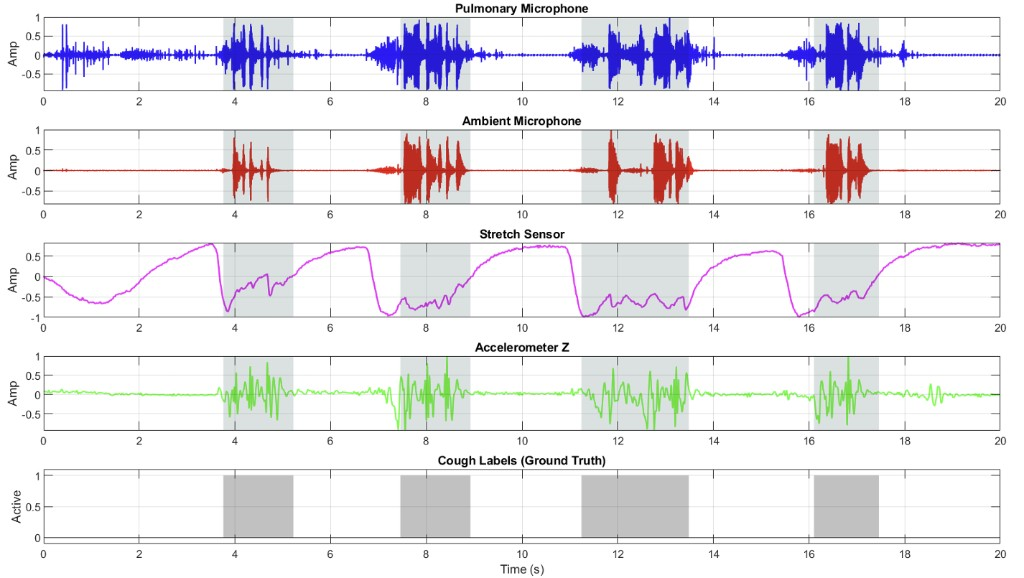
\includegraphics[width=\textwidth]{preprocessed_signals.png}
\caption{Example preprocessed sensor signals and cough labels.}
\label{fig:preprocessed_signals}
\end{figure}

\section{Sensor Configuration}

Each recording contains four synchronized sensor channels sampled at 4800\,Hz. The channels are listed in Table~\ref{tab:sensors}.

\begin{table}[H]
\centering
\caption{Sensor channel configuration.}
\label{tab:sensors}
\begin{tabular}{@{}clp{7cm}@{}}
\toprule
\textbf{Col} & \textbf{Sensor} & \textbf{Description} \\
\midrule
1 & Pulmonary microphone & Captures internal chest sounds related to coughing \\
2 & Ambient microphone & Records environmental audio \\
3 & Stretch sensor (+\,label) & Measures chest wall expansion; also encodes cough label \\
4 & Accelerometer (Z-axis) & Captures vertical body motion \\
\bottomrule
\end{tabular}
\end{table}

\section{Dataset Composition}

The dataset was expanded during this phase to include 85 recordings, up from 60 in the previous phase. Each recording has a fixed duration of approximately 20 seconds. The majority of the recordings (64) come from one primary subject, while the remaining 21 recordings were collected from three additional subjects to begin evaluating cross-subject variability. The recordings cover multiple activity types (sitting, walking, standing, running) and various contexts including clean, cough noise, music noise, sneeze noise, snooze noise, door noise, generic noise, and false-positive non-cough events. The activity and noise distributions are summarized in Table~\ref{tab:dataset_dist}.

\begin{table}[H]
\centering
\caption{Dataset distribution across activities and noise conditions (85 total recordings).}
\label{tab:dataset_dist}
\begin{tabular}{@{}lcccc|c@{}}
\toprule
\textbf{Activity} & \textbf{Clean} & \textbf{CoughNoise} & \textbf{OtherNoise} & \textbf{FalsePositive} & \textbf{Total} \\
\midrule
Sitting    & 19 & 14 & 10 & 0 & 43 \\
Walking    & 7  & 13 & 2  & 0 & 22 \\
Running    & 4  & 0  & 1  & 0 & 5  \\
Standing   & 7  & 2  & 4  & 2 & 15 \\
\midrule
\textbf{Total} & \textbf{37} & \textbf{29} & \textbf{17} & \textbf{2} & \textbf{85} \\
\bottomrule
\end{tabular}
\\[4pt]
\footnotesize\textit{Note: OtherNoise includes music, sneeze, snooze, door, and generic noise conditions. FalsePositive recordings contain non-cough sounds used to test false alarm robustness.}
\end{table}

Given the small number of running and standing recordings, the deep learning experiments handle these classes carefully. In V1, only sitting and walking are used for activity classification. In V2, all four classes are included but results are interpreted with the class imbalance in mind. In V3, the running class is excluded because having only 5 running records makes reliable stratified splitting across train, validation, and test sets impractical.

It should be noted that the overall dataset size of 85 short recordings is a significant limitation for deep learning, which generally benefits from large amounts of training data. The small dataset restricts the model capacity that can be used without overfitting and limits the reliability of performance estimates. In particular, the class imbalance across activities and the limited number of subjects prevent the models from learning generalizable cross-subject patterns. Expanding the dataset with more subjects, longer sessions, and a more balanced activity distribution is a clear priority for future work.

\section{Ground Truth Encoding}

The cough ground truth is embedded within the stretch sensor channel using bitwise encoding. The least significant bit of the raw value represents the cough label, while the remaining bits represent the sensor magnitude:
\begin{align}
y[n] &= x[n] \;\&\; 1 \label{eq:label} \\
s[n] &= x[n] \gg 1 \label{eq:stretch}
\end{align}
where $y[n] = 1$ indicates a cough event and $s[n]$ is the decoded stretch sensor value. This encoding allows both signal and annotation to be stored in a single channel.

\chapter{METHODOLOGY}

\section{Preprocessing}

The preprocessing pipeline is the same as in the first phase (EE491). All recordings are sampled at $F_s = 4800$\,Hz. The following channel-specific filters are applied using 4th-order Butterworth filters with zero-phase (forward--backward) filtering:

\begin{table}[H]
\centering
\caption{Per-channel filter configuration.}
\label{tab:filters}
\begin{tabular}{@{}llll@{}}
\toprule
\textbf{Channel} & \textbf{Filter} & \textbf{Cutoff} & \textbf{Purpose} \\
\midrule
Pulmonary mic & Bandpass & 60--2200\,Hz & Retain cough band, remove drift and hum \\
Ambient mic   & Bandpass & 60--2200\,Hz & Same filter for fair channel comparison \\
Stretch sensor & Low-pass & 20\,Hz & Retain slow chest movement \\
Accelerometer  & Low-pass & 20\,Hz & Preserve DC (gravity) and gross motion \\
\bottomrule
\end{tabular}
\end{table}

Before filtering, the stretch sensor channel is decoded using bitwise operations (Equations~\ref{eq:label}--\ref{eq:stretch}). Audio signals are median-centered. Motion signals (stretch and accelerometer Z-axis) are resampled from 4800\,Hz to 100\,Hz after low-pass filtering.

\section{Windowing and Labeling}

Continuous signals are segmented into overlapping windows of 1.0\,s duration. The window size was chosen to be larger than in the previous phase (200\,ms) to give the CNN models more temporal context. Two labeling strategies were used across the three model versions:

\begin{itemize}[nosep]
    \item \textbf{V1 labeling:} A window is labeled as cough-positive if \emph{any} cough label exists within the full window. The hop size is 0.5\,s.
    \item \textbf{V2/V3 labeling:} A window is labeled as cough-positive only if a cough label exists in the \emph{center 20\%} of the window. The hop size is reduced to 0.25\,s.
\end{itemize}

Figure~\ref{fig:windowing} illustrates the difference between these two strategies.

\begin{figure}[H]
\centering
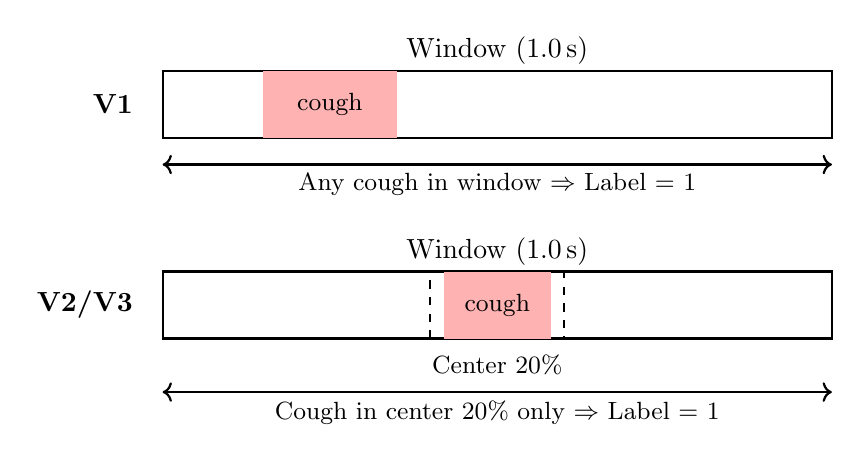
\begin{tikzpicture}[scale=0.85]
    % V1 labeling
    \node[anchor=east] at (-0.3, 1.5) {\textbf{V1}};
    \draw[thick] (0, 1) rectangle (10, 2);
    \node at (5, 2.3) {Window (1.0\,s)};
    \fill[red!30] (1.5, 1) rectangle (3.5, 2);
    \node[font=\small] at (2.5, 1.5) {cough};
    \draw[thick, <->] (0, 0.6) -- (10, 0.6);
    \node[font=\small] at (5, 0.3) {Any cough in window $\Rightarrow$ Label = 1};

    % V2/V3 labeling
    \node[anchor=east] at (-0.3, -1.5) {\textbf{V2/V3}};
    \draw[thick] (0, -2) rectangle (10, -1);
    \node at (5, -0.7) {Window (1.0\,s)};
    \draw[dashed, thick] (4, -2) rectangle (6, -1);
    \node[font=\small] at (5, -2.4) {Center 20\%};
    \fill[red!30] (4.2, -2) rectangle (5.8, -1);
    \node[font=\small] at (5, -1.5) {cough};
    \draw[thick, <->] (0, -2.8) -- (10, -2.8);
    \node[font=\small] at (5, -3.1) {Cough in center 20\% only $\Rightarrow$ Label = 1};
\end{tikzpicture}
\caption{Comparison of V1 and V2/V3 window labeling strategies.}
\label{fig:windowing}
\end{figure}

The center labeling strategy reduces the number of windows that are labeled as positive only because a cough event partially overlaps with the window boundary. This provides cleaner labels for training, at the cost of labeling fewer windows as positive.

Each window produces two input tensors: an audio tensor of shape $(2, 4800)$ containing the pulmonary and ambient microphone signals, and a motion tensor of shape $(2, 100)$ containing the stretch and accelerometer signals.

\section{Model Architecture}

All three model versions follow a dual-branch architecture with late fusion. Two separate CNN branches process the audio and motion inputs independently. Their output embeddings are concatenated and passed through fully connected layers for classification. Figure~\ref{fig:architecture} shows the general architecture.

\begin{figure}[H]
\centering
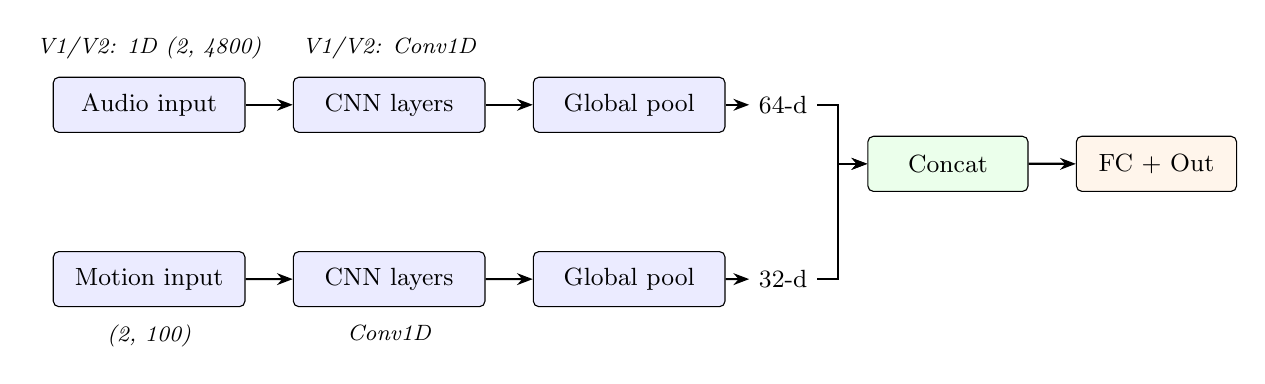
\begin{tikzpicture}[
    block/.style={rectangle, draw, fill=blue!8, text width=2.2cm, text centered, minimum height=0.7cm, rounded corners=2pt, font=\small},
    blockG/.style={rectangle, draw, fill=green!8, text width=1.8cm, text centered, minimum height=0.7cm, rounded corners=2pt, font=\small},
    blockO/.style={rectangle, draw, fill=orange!8, text width=1.8cm, text centered, minimum height=0.7cm, rounded corners=2pt, font=\small},
    arr/.style={-{Stealth[length=2mm]}, thick},
    scale=0.9
]

% Audio branch
\node[block] (ain) {Audio input};
\node[block, right=0.6cm of ain] (acnn) {CNN layers};
\node[block, right=0.6cm of acnn] (apool) {Global pool};
\node[font=\small, right=0.3cm of apool] (adim) {64-d};

% Motion branch
\node[block, below=1.5cm of ain] (min) {Motion input};
\node[block, right=0.6cm of min] (mcnn) {CNN layers};
\node[block, right=0.6cm of mcnn] (mpool) {Global pool};
\node[font=\small, right=0.3cm of mpool] (mdim) {32-d};

% Fusion
\node[blockG, right=1.8cm of apool, yshift=-0.75cm] (cat) {Concat};
\node[blockO, right=0.6cm of cat] (fc) {FC + Out};

% Labels
\node[font=\footnotesize\itshape, above=0.1cm of ain] {V1/V2: 1D (2, 4800)};
\node[font=\footnotesize\itshape, above=0.1cm of acnn] {V1/V2: Conv1D};
\node[font=\footnotesize\itshape, below=0.1cm of min] {(2, 100)};
\node[font=\footnotesize\itshape, below=0.1cm of mcnn] {Conv1D};

% Arrows
\draw[arr] (ain) -- (acnn);
\draw[arr] (acnn) -- (apool);
\draw[arr] (apool) -- (adim);
\draw[arr] (adim.east) -- ++(0.3,0) |- (cat.west);
\draw[arr] (min) -- (mcnn);
\draw[arr] (mcnn) -- (mpool);
\draw[arr] (mpool) -- (mdim);
\draw[arr] (mdim.east) -- ++(0.3,0) |- (cat.west);
\draw[arr] (cat) -- (fc);

\end{tikzpicture}
\caption{General dual-branch architecture with late fusion. V1/V2 use 1D CNNs on raw audio waveforms. V3 replaces the audio branch with a 2D CNN on log-Mel spectrograms.}
\label{fig:architecture}
\end{figure}

\subsection{V1: Dual-Branch 1D CNN}

The V1 model (\texttt{DualBranchCoughCNN}) takes raw waveform inputs. The audio branch processes the 2-channel audio signal through three Conv1D layers with increasing channel counts ($2 \to 16 \to 32 \to 64$), each followed by batch normalization, ReLU, and max pooling. A global adaptive average pooling layer reduces the output to a 64-dimensional embedding.

The motion branch has a similar but smaller structure: two Conv1D layers ($2 \to 16 \to 32$) followed by adaptive average pooling, producing a 32-dimensional embedding.

The two embeddings are concatenated (96 dimensions) and passed through a classifier: Linear($96 \to 64$) $\to$ ReLU $\to$ Dropout(0.3) $\to$ Linear($64 \to 1$). The output is a single logit for binary cough detection.

\subsection{V2: Enhanced Training Strategy}

The V2 model uses the same \texttt{DualBranchCoughCNN} architecture as V1. The improvements are in the training process:

\begin{itemize}[nosep]
    \item \textbf{Data augmentation:} Additive white Gaussian noise (AWGN) is applied to both audio and motion tensors during cough detection training. For activity classification (Phase~2), synchronized circular time shifts are additionally applied.
    \item \textbf{Learning rate scheduling:} \texttt{ReduceLROnPlateau} monitors the validation loss and reduces the learning rate by half after 3 epochs without improvement.
    \item \textbf{Center labeling:} As described in Section~4.2, only cough labels in the center 20\% of the window count as positive.
    \item \textbf{Longer training:} The number of epochs is increased from 15 to 25.
\end{itemize}

\subsection{V3: Spectrogram-Based Model}

The V3 model (\texttt{Spec2DCoughCNN}) changes the audio input from raw waveforms to log-Mel spectrograms. The spectrogram is computed using the following parameters:

\begin{itemize}[nosep]
    \item FFT size: $N_{\text{FFT}} = 512$
    \item Hop length: 128 samples
    \item Mel bands: $N_{\text{MELS}} = 64$
    \item Frequency range: 60--2200\,Hz (matching the audio bandpass filter)
\end{itemize}

The resulting spectrogram has shape $(2, 64, 38)$ for 2 channels, 64 Mel bands, and 38 time frames per 1-second window. A logarithmic transformation is applied: $\log(\text{mel} + 10^{-9})$.

The audio branch uses three Conv2D layers ($2 \to 16 \to 32 \to 64$ channels) with $3 \times 3$ kernels, batch normalization, ReLU, and max pooling. Adaptive average pooling produces a 64-dimensional embedding. The motion branch remains unchanged from V1/V2.

An example log-Mel spectrogram is shown in Figure~\ref{fig:melspec}.

\begin{figure}[H]
\centering
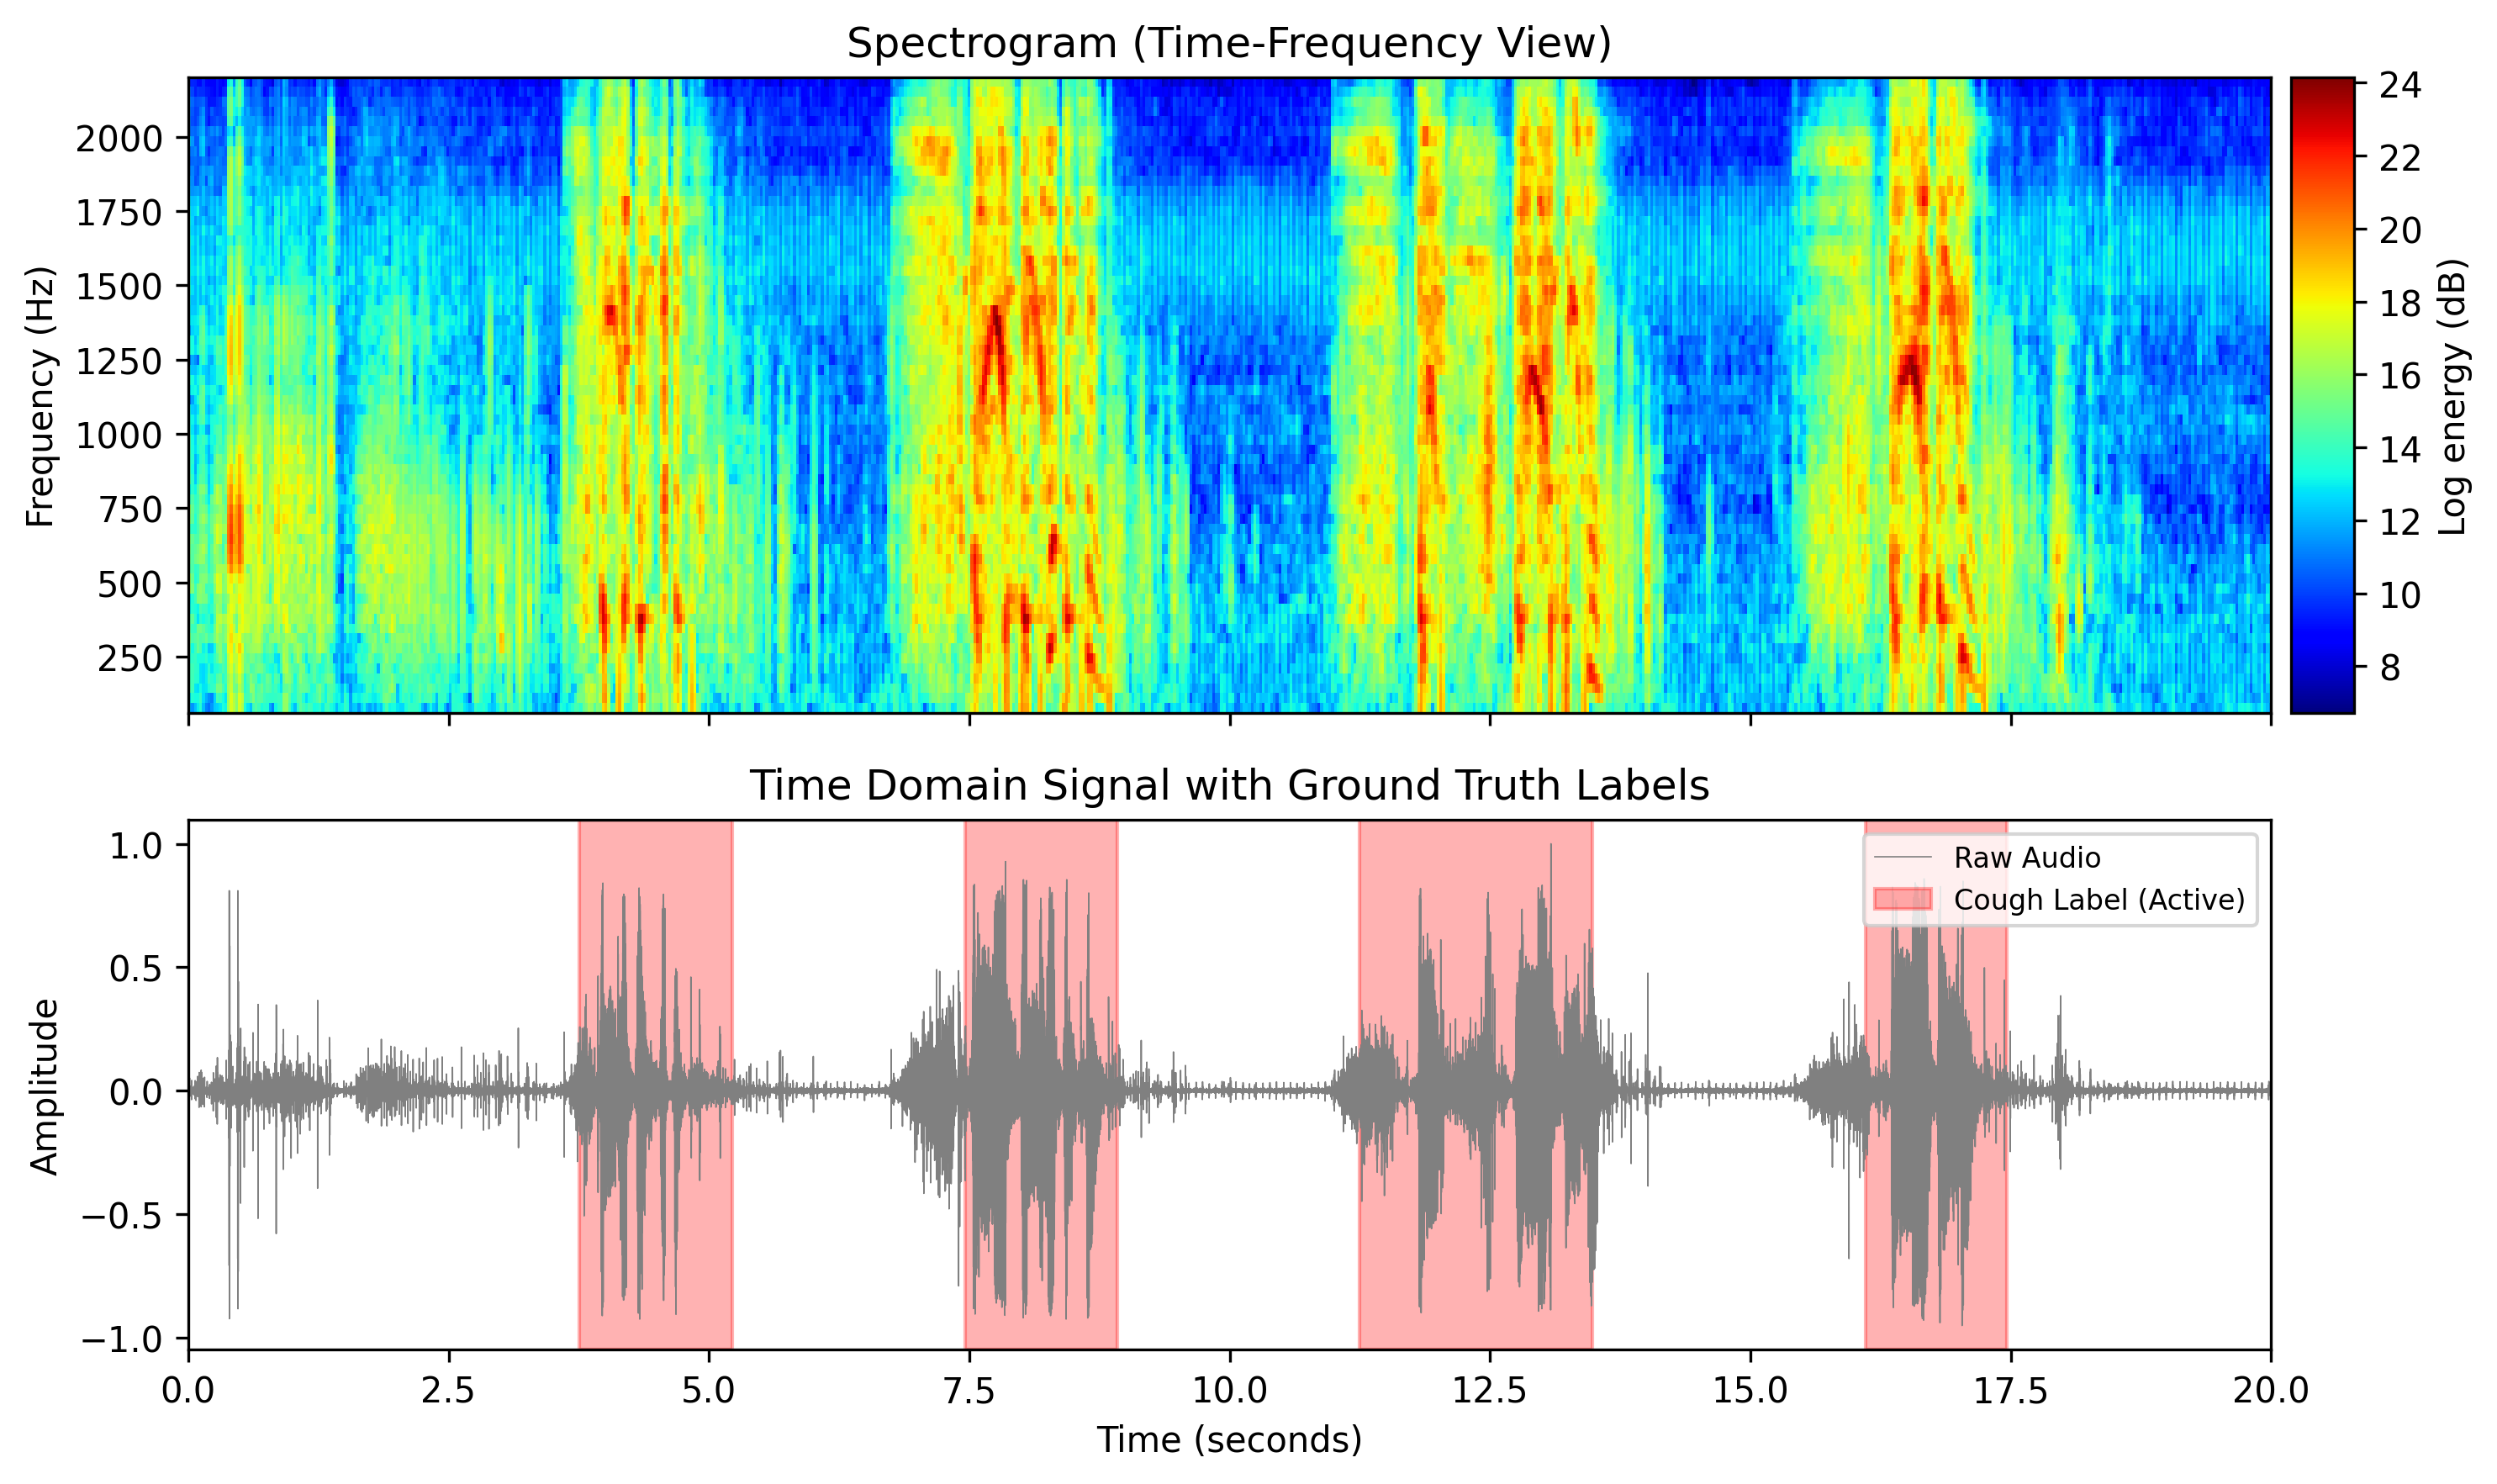
\includegraphics[width=0.8\textwidth]{mel_spectrogram_example.png}
\caption{Example log-Mel spectrogram of the pulmonary microphone channel (top) and the corresponding time-domain signal with ground truth cough labels (bottom). Cough events appear as broadband vertical patterns in the spectrogram.}
\label{fig:melspec}
\end{figure}

\section{Training Configuration}

Table~\ref{tab:training_config} summarizes the training configuration for Phase~1 (cough detection) across all three versions.

\begin{table}[H]
\centering
\caption{Phase~1 (cough detection) training configuration comparison.}
\label{tab:training_config}
\small
\begin{tabular}{@{}lccc@{}}
\toprule
\textbf{Parameter} & \textbf{V1} & \textbf{V2} & \textbf{V3} \\
\midrule
Audio input & Raw waveform & Raw waveform & Log-Mel spectrogram \\
Audio CNN & 1D & 1D & 2D \\
Window / hop (s) & 1.0\,/\,0.5 & 1.0\,/\,0.25 & 1.0\,/\,0.25 \\
Label rule & Full window & Center 20\% & Center 20\% \\
Optimizer & Adam & Adam & Adam \\
Learning rate & $10^{-3}$ & $10^{-3}$ & $10^{-3}$ \\
Weight decay & $10^{-4}$ & $10^{-4}$ & $10^{-4}$ \\
Epochs & 15 & 25 & 25 \\
Batch size & 64 & 64 & 64 \\
Loss & \multicolumn{3}{c}{BCEWithLogitsLoss} \\
\texttt{pos\_weight} & $\sim$3.1 & $\sim$4.8 & $\sim$4.8 \\
Augmentation & None & AWGN & None \\
LR scheduler & None & \multicolumn{2}{c}{ReduceLROnPlateau} \\
\bottomrule
\end{tabular}
\end{table}

All three versions use the Adam optimizer~\cite{kingma2015adam} with binary cross-entropy loss (BCEWithLogitsLoss)~\cite{goodfellow2016deep} for cough detection. The \texttt{pos\_weight} parameter compensates for class imbalance by weighting positive (cough) samples more in the loss function. It is computed as the ratio of negative to positive training windows. The higher value in V2/V3 reflects the stricter center labeling, which produces fewer positive windows.

\section{Activity Classification (Phase 2)}

After cough detection, a second model is trained for activity classification using the same dual-branch architecture but with a multi-class output head.

\begin{itemize}[nosep]
    \item \textbf{V1:} Only 2 classes (sitting and walking) are used. Only windows from cough-positive segments are included. The loss is cross-entropy~\cite{goodfellow2016deep}.
    \item \textbf{V2:} All 4 activity classes (sitting, walking, standing, running) are used. All windows are included regardless of cough presence. The loss is weighted cross-entropy with class weights, using AdamW optimizer~\cite{loshchilov2019adamw}.
    \item \textbf{V3:} Three activity classes (sitting, standing, walking) are used. Running is excluded because having only 5 running records makes reliable stratified splitting across train, validation, and test sets impractical. Stratified record-level splitting is applied to ensure balanced activity representation. Multiple runs (A--D) are conducted with different combinations of class weighting and weighted sampling to find the best configuration.
\end{itemize}

\section{Validation Strategy}

For Phase~1 (cough detection), data is split at the record level into training (70\%), validation (15\%), and test (15\%) sets using random splitting. This ensures that windows from the same recording do not appear in different splits. V1 used 71 records (train~49 / val~11 / test~11), while V2 and V3 used 85 records (train~59 / val~13 / test~13).

Unlike the GroupKFold cross-validation used in EE491, a single train/val/test split is used here. This choice is motivated by the higher computational cost of deep learning training, which makes repeated cross-validation impractical.

For Phase~2 (activity classification) in V3, a stratified split is applied based on record-level activity labels to ensure that each split contains a representative distribution of activities.

\chapter{IMPLEMENTATION AND RESULTS}

This chapter presents the experimental results for both cough detection and activity classification across all three model versions. All metrics are computed on held-out test sets that contain no recordings from the training or validation sets.

\section{Cough Detection Results}

\subsection{Performance Comparison}

Table~\ref{tab:cough_results} compares the cough detection test results across V1, V2, and V3.

\begin{table}[H]
\centering
\caption{Test set cough detection performance across model versions.}
\label{tab:cough_results}
\begin{tabular}{@{}lccc@{}}
\toprule
\textbf{Metric} & \textbf{V1} & \textbf{V2} & \textbf{V3} \\
\midrule
Test windows & 429 & 1001 & 1001 \\
Cough windows (\%) & 129 (30.1\%) & 192 (19.2\%) & 192 (19.2\%) \\
\midrule
Overall accuracy & 0.89 & 0.91 & 0.93 \\
\midrule
Non-cough precision & 0.89 & 0.98 & 0.99 \\
Non-cough recall & 0.96 & 0.91 & 0.92 \\
Non-cough F1 & 0.92 & 0.94 & 0.95 \\
\midrule
Cough precision & 0.89 & 0.71 & 0.74 \\
Cough recall & 0.71 & 0.92 & 0.95 \\
Cough F1 & 0.79 & 0.80 & 0.83 \\
\bottomrule
\end{tabular}
\end{table}

\textbf{Important note on comparability:} V1 uses a different labeling strategy (full-window) and hop size (0.5\,s) than V2/V3 (center-20\% labeling, 0.25\,s hop). V1 also uses fewer records (71 vs.\ 85). As a result, the V1 test set has different characteristics, and direct numerical comparison with V2/V3 should be interpreted carefully.

\subsection{Confusion Matrix Analysis}

Figure~\ref{fig:cough_cm} shows the confusion matrices for the cough detection test sets.

\begin{figure}[H]
\centering
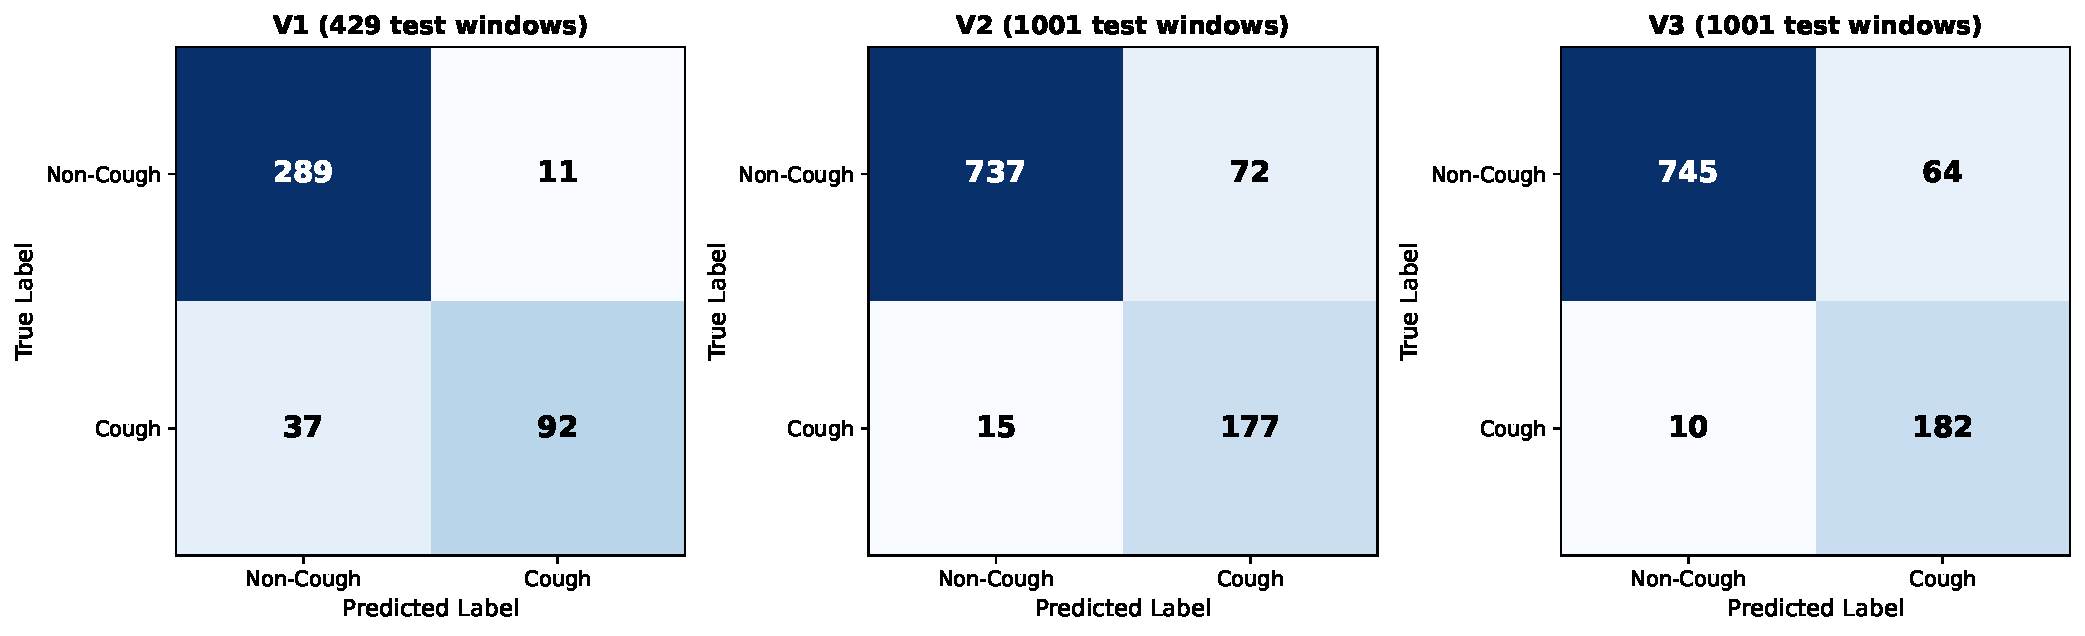
\includegraphics[width=\textwidth]{cough_confusion_matrices.pdf}
\caption{Cough detection confusion matrices for V1 (left), V2 (center), and V3 (right).}
\label{fig:cough_cm}
\end{figure}

\subsection{Discussion}

The results show a clear progression from V1 to V3:

\begin{itemize}[nosep]
    \item \textbf{V1 to V2:} Cough recall improves from 0.71 to 0.92. This is likely due to the combination of center labeling (which gives cleaner ground truth), data augmentation (which improves generalization), and learning rate scheduling. However, cough precision drops from 0.89 to 0.71, meaning more false alarms occur.
    \item \textbf{V2 to V3:} Cough recall further improves from 0.92 to 0.95, and cough precision increases slightly from 0.71 to 0.74. The log-Mel spectrogram representation allows the 2D CNN to capture frequency patterns that distinguish coughs from other sounds.
\end{itemize}

Across all versions, the models successfully avoid predicting only the majority class. This confirms that the class weighting (\texttt{pos\_weight}) in the loss function is effective.

\section{Activity Classification Results}

Table~\ref{tab:activity_results} summarizes the activity classification results.

\begin{table}[H]
\centering
\caption{Activity classification test results across model versions.}
\label{tab:activity_results}
\begin{tabular}{@{}lccc@{}}
\toprule
\textbf{} & \textbf{V1} & \textbf{V2} & \textbf{V3 (Run-B)} \\
\midrule
Number of classes & 2 & 4 & 3 \\
Windows used & Cough-only & All & All \\
Test accuracy & 0.96 & 0.66 & 0.92 \\
Macro F1 & -- & -- & 0.91 \\
\bottomrule
\end{tabular}
\end{table}

\textbf{V1:} Activity classification used only 2 classes (sitting and walking) and only windows from cough segments. The test set contained 100 sitting and only 4 walking test windows, so the high accuracy of 0.96 is not reliable due to the extreme class imbalance in the test data.

\textbf{V2:} All 4 activity classes were used with all windows. The overall accuracy of 0.66 reflects the difficulty of the 4-class problem, especially with imbalanced class distributions. The test set had no running samples at all, which made the running class metrics meaningless.

\textbf{V3:} Multiple training runs (A--D) were compared by varying class weighting and weighted sampling strategies. A walking recall guardrail was applied: any run whose walking recall drops more than 0.05 compared to the baseline (Run-A) is penalized. Among the runs that pass, the one with the highest standing recall and macro F1 is selected.

\begin{itemize}[nosep]
    \item Run-A (baseline): No class weighting or sampling. Overall accuracy 0.84, walking recall 0.77.
    \item Run-B (class weights): Class weights in the loss function. Overall accuracy 0.92, walking recall 0.81, macro F1 0.91.
    \item Run-C (weighted sampler): Weighted random sampling during training. Overall accuracy 0.87, walking recall 0.78.
    \item Run-D (weights + sampler): Both class weights and weighted random sampling. Overall accuracy 0.88, walking recall 0.85.
\end{itemize}

All four runs passed the walking recall guardrail. Run-B was selected as the best configuration because it achieved the highest standing recall (0.86) and macro F1 (0.91) among all passing runs.

\section{Comparison with Classical ML}

Table~\ref{tab:ml_comparison} provides a brief comparison between the deep learning results and the classical ML results from EE491.

\begin{table}[H]
\centering
\caption{Comparison of DL (this work) and classical ML (EE491) cough detection.}
\label{tab:ml_comparison}
\begin{tabular}{@{}lcc@{}}
\toprule
\textbf{Aspect} & \textbf{Classical ML (EE491)} & \textbf{DL -- V3 (this work)} \\
\midrule
Features & Handcrafted (8 features) & Learned (CNN) \\
Audio input & Time/freq statistics & Log-Mel spectrogram \\
Window size & 200\,ms & 1000\,ms \\
Validation & GroupKFold (5 folds) & Single split (70/15/15) \\
Best window F1 (cough) & 0.83 (RF) & 0.83 (V3) \\
Event-level F1 & 0.92 (XGBoost) & Not yet evaluated \\
\midrule
Activity accuracy & 0.89 (2-class) & 0.92 (3-class, V3 Run-B) \\
\bottomrule
\end{tabular}
\end{table}

The window-level cough F1 scores are similar between the best classical ML model and V3. However, the DL approach does not require manual feature engineering and works with a larger window size. Event-level evaluation, which was a key metric in EE491, has not yet been applied to the DL models. This is an important direction for future work.

The activity classification comparison is also not straightforward, as EE491 used 2 classes while V3 uses 3 classes (running excluded). The higher accuracy of V3 on a harder problem is encouraging.

\section{Qualitative Analysis}

Figure~\ref{fig:prediction_timeline} shows a time-aligned visualization of V3 predictions on a test recording. The model produces high cough probabilities during actual cough events and low probabilities during non-cough regions.

\begin{figure}[H]
\centering
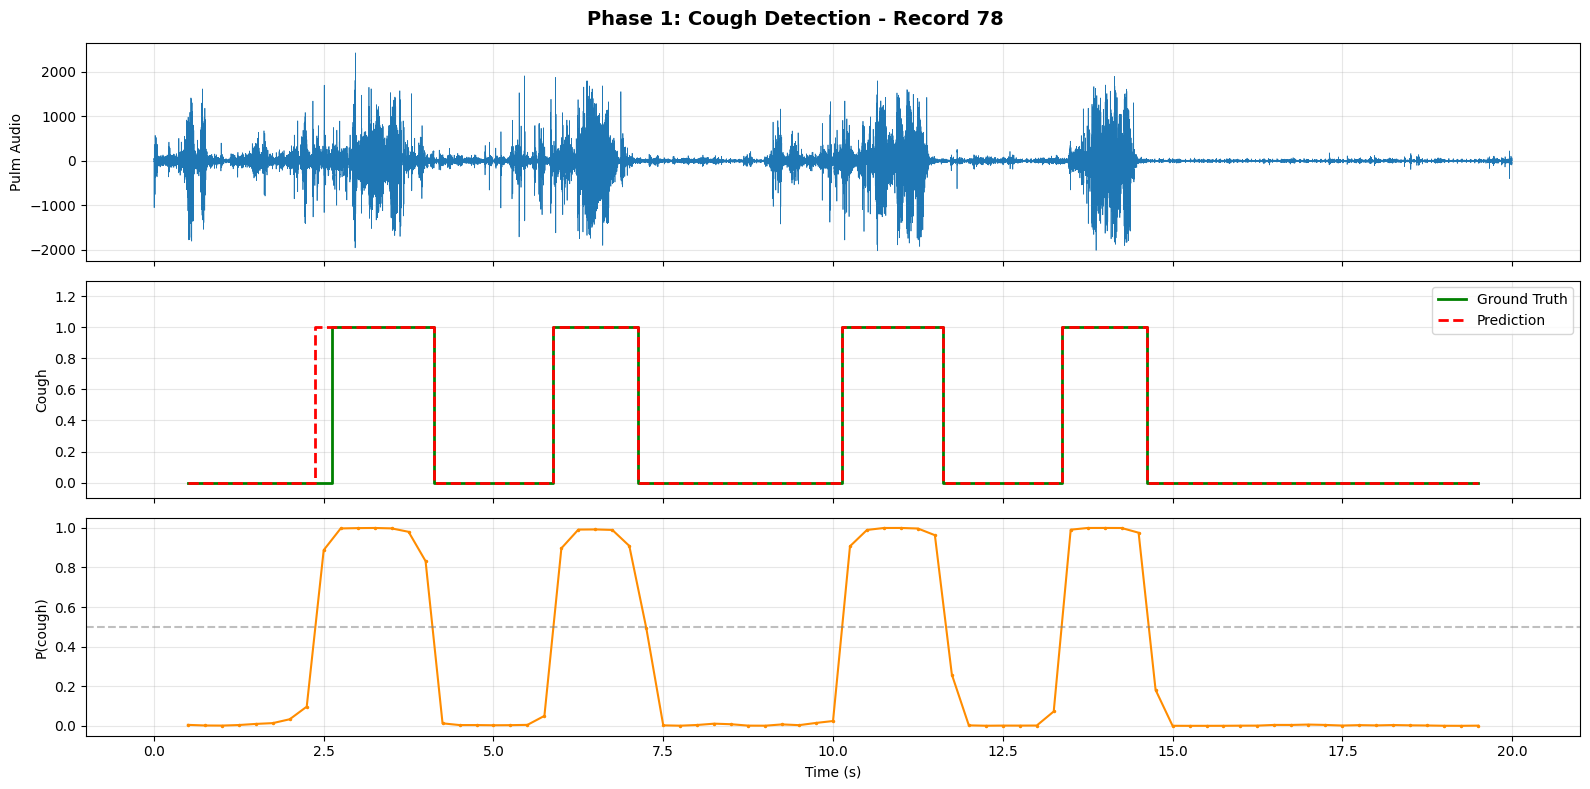
\includegraphics[width=\textwidth]{prediction_timeline.png}
\caption{V3 prediction timeline on a test recording. Top: preprocessed audio signal. Middle: ground-truth cough labels. Bottom: predicted cough probability over time.}
\label{fig:prediction_timeline}
\end{figure}

\chapter{CONCLUSION}

\section{Summary}

In this work, three deep learning model versions were developed for cough detection and activity classification using wearable multi-sensor data. The models follow a dual-branch CNN architecture that processes audio and motion signals separately and combines them through late fusion.

The first version (V1) established a baseline using raw 1D waveform inputs. The second version (V2) improved training through center-focused window labeling, data augmentation, and learning rate scheduling. The third version (V3) replaced the raw audio input with log-Mel spectrograms processed by a 2D CNN, which achieved the best overall performance.

For cough detection, V3 achieved 0.93 overall accuracy with 0.95 cough recall and 0.74 cough precision on the test set. Compared to V1, cough recall improved from 0.71 to 0.95 across the three versions. For activity classification, V3 reached 0.92 accuracy and 0.91 macro F1-score on a 3-class problem (sitting, standing, walking) using class weighting.

These results show that deep learning models can effectively detect coughs from multi-sensor wearable data without relying on handcrafted features.

\section{Future Work}

Several directions are identified for future work:

\begin{itemize}[nosep]
    \item \textbf{Event-level evaluation:} Applying the IoU-based event-level evaluation from EE491 to the deep learning models would allow a more direct comparison with classical ML methods.
    \item \textbf{More data:} The current dataset of 85 short recordings from a limited number of subjects is small for deep learning. This restricts model capacity, reduces the reliability of performance estimates, and prevents evaluation of cross-subject generalization. Expanding the dataset with more subjects, longer recording sessions, and a more balanced distribution of activities and noise conditions is the most important next step.
    \item \textbf{Threshold tuning:} The current decision threshold is fixed at 0.5. Tuning this threshold based on the precision--recall trade-off could improve practical performance.
    \item \textbf{Model refinement:} Exploring architectures such as recurrent neural networks or attention mechanisms, and applying more systematic hyperparameter tuning, could improve results.
    \item \textbf{Real-time operation:} The current system is designed for offline analysis. Adapting the pipeline for real-time or near-real-time use would require causal filtering and efficient inference.
\end{itemize}

\section{Realistic Constraints}

\subsection{Social, Environmental and Economic Impact}

The primary social value of this project is its potential for health monitoring. A reliable cough detection system may support long-term respiratory monitoring and provide useful information for clinicians. However, the current system is a prototype and is not intended for clinical diagnosis. The project uses low-power wearable sensors and software-based analysis, so its environmental impact is minimal.

\subsection{Cost Analysis}

The primary cost is labor. Assuming approximately 10 hours per week during the semester at an hourly rate of \$15, the labor cost for two semesters is estimated at \$4800. Since the sensing hardware and data acquisition system are already available in the laboratory, no additional hardware costs are incurred.

\subsection{Standards}

If extended toward clinical use, the system should comply with relevant medical device standards such as ISO/IEEE 11073 for communication and interoperability, and IEEE 12207 for software life cycle management. Compliance with Turkish and European Union medical device regulations (MDR) would also be required.


% ---- Bibliography ----

\begin{thebibliography}{}

\bibitem{dixon2025}
Dixon, P. C., Dubeau, S., Roy, J.-F., \& Fournier, P.-A. (2025).
Automatic cough detection via a multi-sensor smart garment using machine learning.
\textit{Computers in Biology and Medicine}, \textit{191}, 110192.

\bibitem{elfaramawy2017}
T.~Elfaramawy, C.~Latyr~Fall, M.~Morissette, F.~Lellouche, and B.~Gosselin,
``Wireless respiratory monitoring and coughing detection using a wearable patch sensor network,''
in \textit{Proc. 15th IEEE Int. New Circuits and Systems Conf. (NEWCAS)},
Strasbourg, France, 2017, pp.~197--200, doi:~10.1109/NEWCAS.2017.8010139.

\bibitem{bales2020}
Bales, C., Nabeel, M., John, C. N., Masood, U., Qureshi, H. N., Farooq, H., Posokhova, I., \& Imran, A. (2020).
Can machine learning be used to recognize and diagnose coughs?
In \textit{Proceedings of the International Conference on e-Health and Bioengineering (EHB)} (pp. 1--4).
IEEE.
https://doi.org/10.1109/EHB50910.2020.9280115

\bibitem{amoh2016}
Amoh, J., \& Odame, K. (2016).
Deep neural networks for identifying cough sounds.
\textit{IEEE Transactions on Biomedical Circuits and Systems}, \textit{10}(5), 1003--1011.
https://doi.org/10.1109/TBCAS.2016.2598794

\bibitem{otoshi2021}
T.~Otoshi, T.~Nagano, S.~Izumi, D.~Hazama, \textit{et~al.}, ``A novel automatic cough frequency monitoring system combining a triaxial accelerometer and a stretchable strain sensor,'' \textit{Sci. Rep.}, vol.~11, Art.~no.~9973, 2021.
https://doi.org/10.1038/s41598-021-89457-0

\bibitem{shi2018}
Y.~Shi, H.~Liu, Y.~Wang, M.~Cai, and W.~Xu, ``Theory and application of audio-based assessment of cough,'' \textit{J. Sensors}, vol.~2018, Art.~no.~9845321, 2018.
https://doi.org/10.1155/2018/9845321

\bibitem{sanchezmorillo2024}
D.~Sanchez Morillo, D.~Sales Lerida, B.~Priego Torres, and A.~Le\'on Jim\'enez, ``Cough detection using acceleration signals and deep learning techniques,'' \textit{Electronics}, vol.~13, no.~12, Art.~no.~2410, 2024.
https://doi.org/10.3390/electronics13122410

\bibitem{kingma2015adam}
D.~P.~Kingma and J.~Ba, ``Adam: A method for stochastic optimization,'' in \textit{Proc. 3rd Int. Conf. Learning Representations (ICLR)}, San Diego, CA, USA, 2015.
https://arxiv.org/abs/1412.6980

\bibitem{loshchilov2019adamw}
I.~Loshchilov and F.~Hutter, ``Decoupled weight decay regularization,'' in \textit{Proc. 7th Int. Conf. Learning Representations (ICLR)}, New Orleans, LA, USA, 2019.
https://arxiv.org/abs/1711.05101

\bibitem{goodfellow2016deep}
I.~Goodfellow, Y.~Bengio, and A.~Courville, \textit{Deep Learning}.\hspace{0.5em}Cambridge, MA: MIT Press, 2016.
https://www.deeplearningbook.org/

\end{thebibliography}

\end{document}
